\chapter{Аналитический раздел}

В данном разделе представлена основная информация об очереди и реализациях очереди в виде массива и линейного односвязного списка.

\section{Теоритические сведения}

Очередь  – это  последовательный  список  переменной  длины,  включение 
элементов в который идет с одной стороны (с «хвоста»), а исключение –  с другой 
стороны (с «головы»). Принцип работы очереди: первым пришел – первым вышел, т. 
е. \textit{First In – First Out (FIFO)}. 
Для «хвоста» и «головы» очереди используют соответственно два указателя \textit{Pin} 
и \textit{Pout}, то есть, исключается элемент с адресом \textit{Pout} и включается элемент по адресу 
\textit{Pin}.

\section{Реализации очереди}

Моделировать  простейшую  линейную  очередь  можно  как  на  основе  вектора 
(одномерного массива), так и на основе динамического списка.

\subsection{В виде массива}

При  моделировании  простейшей 
линейной  очереди  на  основе  одномерного  массива  выделяется  последовательная 
область памяти из $m$ мест по $L$ байт, где $L$ – размер поля данных для одного элемента 
размещаемого типа. В каждый текущий момент времени выделенная память может 
быть вся свободна, занята частично или занята полностью. 
В  начале  процесса  очередь  пуста,  при  этом:  $P_{in}  =  P_{out}  = Q_1$,  где  $Q_1$  –  адрес 
(индекс) первого элемента очереди, а количество элементов очереди (K) равно нулю. 
При включении очередного элемента в очередь он располагается по адресу $P_{in}$, а сам 
указатель $P_{in}$  перемещается на длину типа данных к началу следующего элемента.

\subsection{В виде линейного списка}

Большинство  проблем, 
возникающих при реализации очереди в виде массива, устраняется при реализации 
очереди  на  основе  односвязного  линейного списка,  каждый  элемент  которого 
содержит  информационное  поле  и  поле  с  указателем  «вперед»  (на  следующий 
элемент).  В этом случае в статической памяти можно либо хранить адрес начала и 
конца  очереди,  либо  –  адрес  начала  очереди  и  количество  элементов.  Исходное 
состояние очереди: $Pout = Pin$  - пустой указатель, $K = 0$. 

\section{Описание условия задачи}

Большинство  проблем, 
возникающих при реализации очереди в виде массива, устраняется при реализации 
очереди  на  основе  односвязного  линейного списка,  каждый  элемент  которого 
содержит  информационное  поле  и  поле  с  указателем  «вперед»  (на  следующий 
элемент).  В этом случае в статической памяти можно либо хранить адрес начала и 
конца  очереди,  либо  –  адрес  начала  очереди  и  количество  элементов.  Исходное 
состояние очереди: $Pout = Pin$  - пустой указатель, $K = 0$.

Требуется смоделировать процесс обслуживания первых 1000 заявок первого 
типа, выдавая после обслуживания каждых 100 заявок первого типа информацию о 
текущей и средней длине каждой очереди и о среднем времени пребывания заявок 
каждого типа в очереди. В конце процесса необходимо выдать на экран общее время 
моделирования, время простоя ОА, количество вошедших в систему и вышедших из 
нее заявок первого и второго типов.

\subsection{Техническое задание}

Система  массового  обслуживания  состоит  из  обслуживающего  аппарата 
(ОА) и очереди заявок двух типов. (рисунок \ref{fig:oa})

\begin{figure}
	\centering
	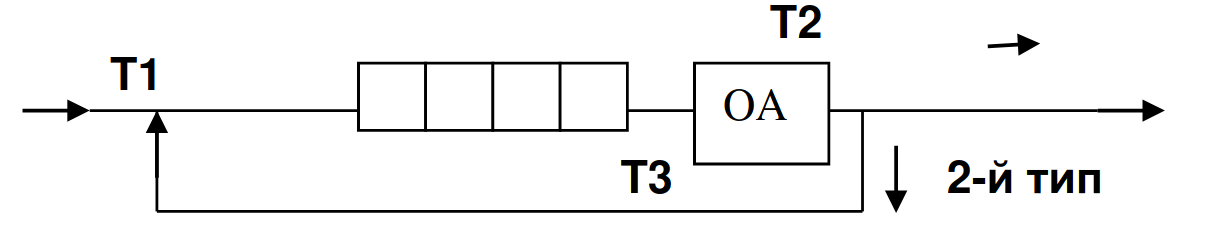
\includegraphics[width=0.7\linewidth]{img/OA}
	\caption{Система массового обслуживания}
	\label{fig:oa}
\end{figure}

Заявки  1-го  типа  поступают  в  "хвост"  очереди  по  случайному  закону  с 
интервалом  времени  Т1, равномерно  распределенным  от  0  до  5 единиц 
времени  (е.в.).  В  ОА  они  поступают  из  "головы"  очереди  по  одной  и 
обслуживаются  также  равновероятно  за  время  Т2  от  0  до  4  е.в.,  после  чего 
покидают систему. 
Единственная  заявка  2-го  типа  постоянно  обращается  в  системе, 
обслуживаясь в ОА равновероятно за время Т3 от 0 до 4 е.в. и возвращаясь в 
очередь не далее 4-й позиции от "головы". В начале процесса заявка 2-го типа 
входит в ОА, оставляя пустую очередь (все времена – вещественного типа). 
Смоделировать  процесс  обслуживания  первых  1000  заявок  1-го  типа. 
Выдавать  после  обслуживания  каждых  100  заявок  1-го  типа  информацию  о 
текущей и средней длине очереди, количестве вошедших и вышедших заявок и 
о  среднем  времени  пребывания  заявок  в  очереди.  В  конце  процесса  выдать 
общее время моделирования, время простоя аппарата, количество вошедших в 
систему  и  вышедших  из  нее  заявок  первого  типа  и  количество  обращений 
заявок  второго  типа.  По  требованию  пользователя  выдать  на  экран  адреса 
элементов  очереди  при  удалении  и  добавлении  элементов.  Проследить, 
возникает ли при этом фрагментация памяти.

\section{Вывод}

В данном разделе были рассмотрены основные теоритические сведения об очередях и реализациях очередей, а также сформулировано техническое задание.

\chapter{Конструкторский раздел}

В данном разделе будут описаны используемые структуры данных, приведен список функций для работы с ними, а также описан алгоритм моделирования работы ОА и теоритически рассчитаны результаты работы модели.

\section{Описание структур данных}

Ниже, на листинге \ref{lst:qarr}, представлена структура очереди, реализованная на основе (кольцевого) массива, и функции для работы с данной структурой.

\begin{lstlisting}[language=C,caption=Структура очереди на массиве,label=lst:qarr]
typedef struct
{
	uint32_t size;      // Размер очереди
	uint32_t capacity;  // Вместимость очереди
	request_t *begin;   // Начало массива, выделенного под очередь
	request_t *first;   // "Хвост" очереди
	request_t *last;    // "Голова" очереди
} qarr_t;

// Выделение памяти под пустую очередь
qarr_t qarr_create(uint32_t size);

// Очищение памяти под очередь
void qarr_destroy(qarr_t *queue);

// Вставка элемента в "хвост" очереди
int qarr_push_back(qarr_t *queue, request_t value);

// Вставка элемента в очередь
int qarr_insert(qarr_t *queue, uint32_t pos, request_t value);

// Удаление элемента из "головы" очереди
int qarr_pop_front(qarr_t *queue, request_t *value);

// Печать очереди на экран
void qarr_print(const qarr_t *queue);
\end{lstlisting}

Ниже, на листинге \ref{lst:qlist}, представлена структура очереди, реализованная на основе линейного односвязного списка, и функции для работы с ней.

\begin{lstlisting}[language=C,caption=Структура очереди на линейном списке,label=lst:qlist]
typedef struct node
{
	request_t data;     // Запрос ОА
	struct node *next;  // Следующий узел
} node_t;


typedef struct
{
	uint32_t size;  // Размер очереди
	node_t *first;  // "Хвост" очереди
	node_t *last;   // "Голова" очереди
} qlist_t;


// Создание пустой очереди
qlist_t qlist_create(void);

// Очищение памяти под очередь
void qlist_destroy(qlist_t *queue);

// Вставка элемента в "хвост" очереди
int qlist_push_back(qlist_t *queue, request_t value);

// Вставка элемента в очередь
int qlist_insert(qlist_t *queue, uint32_t pos, request_t value);

// Удаление элемента из "головы" очереди
int qlist_pop_front(qlist_t *queue, request_t *value);

// Печать очереди на экран
void qlist_print(const qlist_t *queue);
\end{lstlisting}

Ниже, на листинге \ref{lst:uni}, представлена структура, являющаяся <<оберткой>> над структурами очередей, реализованных на основе массива и линейного односвязного списка, позволяющая работать с двумя структурами, используя один набор функций.

\begin{lstlisting}[language=C,caption=Универсальная структура очереди,label=lst:uni]
/**
* Реализация очереди:
* ARRAY_QUEUE - через массив
* LIST_QUEUE  - через линейный односвязный список
*/
typedef enum 
{
	ARRAY_QUEUE,
	LIST_QUEUE
} qtype_t;


/**
* @brief Структура очереди
* 
*/
typedef struct
{
	qtype_t type;       // Реализация очереди
	
	union
	{
		qlist_t lst;    // Очередь на списке
		qarr_t arr;     // Очередь на массиве
	} imp;

} queue_t;

/**
* @brief Создание пустой очереди
* 
* \param[in] type тип очереди (ARRAY_QUEUE или LIST_QUEUE)
* \param[in] size вместимость очереди (для ARRAY_QUEUE)
* 
* \return Возвращается очередь: выделенная память под очередь 
* на массиве или пустая очередь на списке
*/
queue_t queue_create(qtype_t type, uint32_t size);

/**
* @brief Очищение памяти, занимаемой очередью
* 
* @param queue очередь, память из-под которой следует очистить
*/
void queue_destroy(queue_t *queue);

/**
* @brief Вставка элемента в "хвост" очереди
* 
* @param queue очередь, в которую вставляется элемент
* @param value элемент для вставки
* @return код ошибки: 0 при успешном завершении.
*/
int queue_push_back(queue_t *queue, request_t value);

/**
* @brief Вставка элемента в очередь
* 
* @param queue очередь, в которую вставляется элемент
* @param pos позиция для вставки (отсчитывается от головы)
* @param value элемент для вставки
* @return код ошибки: 0 при успешном завершении.
*/
int queue_insert(queue_t *queue, uint32_t pos, request_t value);

/**
* @brief Удаление элемента из "головы" очереди
* 
* @param queue очередь, из которой удаляется элемент
* @param value значение удаляемого элемента
* @return код ошибки: 0 при успешном завершении.
*/
int queue_pop_front(queue_t *queue, request_t *value);

/**
* @brief Печатает очередь в stdout
* 
* @param queue очередь для печати
*/
void queue_print(const queue_t *queue);

/**
* @brief Заполняет
* 
* @param queue 
* @param n 
* @return int 
*/
int queue_fill(queue_t *queue, const int n);
\end{lstlisting}

\section{Описание алгоритма}

\textbf{Алгоритм моделирования:}

\begin{enumerate}
	\item Выбрать ближайшее событие (по времени) из следующих:
	\begin{enumerate}
		\item Приход заявки 1-го типа.
		\item Завершение обработки текущей заявки аппаратом.
	\end{enumerate}
	\item Реализовать выбранное событие.
	\item Увеличить счётчик времени.
	\item Уменьшить времена next\_request\_1\_time и oa\_time.
	\item Рассчитать новое время до следующего события того же типа.
\end{enumerate}

\clearpage

\section{Теоретический расчет работы ОА}

Ожидаемое время прихода заявок рассчитывается по формуле (2.1):

\begin{equation}
T_{in} = \langle T_1 \rangle \times N = \frac{t_2^{in} - t_1^{in}}{2} \times N
\end{equation}

Подставляя в формулу (2.1) интервал прихода заявки второго типа -- $0\dots5$, получаем: $T_{in} = 2500$ е.в.

Ожидаемое время обработки заявок рассчитывается по формуле (2.2):

\begin{equation}
T_{out} = \langle T_2 \rangle \times N = \frac{t_2^{out} - t_1^{out}}{2} \times N
\end{equation}

Подставляя в формулу (2.2) интервал обработки заявки: -- $0\dots4$, получаем: $T_{out} = 2000$ е.в.

\section{Вывод}

В данном разделе были описаны используемые структуры данных, приведен список функций для работы с ними, а также описан алгоритм моделирования работы ОА и теоритически рассчитаны результаты работы модели.

\chapter{Технологический раздел}

В данном разделе будут представлены листинги кодов реализации моделирования работы ОА, представлены требования к ПО и приведены тестовые данные.

\section{Требования к ПО}

К разрабатываемому ПО предъявлены следующие требования:

\begin{itemize}[$\bullet$]
	\item на вход программе подается режим работы ПО (пункт меню: $0\dots2$);
	\begin{itemize}[---]
		\item если режим работы программы 0 -- производится выход;
		\item если режим работы программы 1 -- производится моделирование работы ОА. На вход в данном режиме подается пункт меню (0 -- выход):
		\begin{enumerate}
			\item Запуск моделирования с параметрами по-умолчанию.
			\item Измененение времени прихода и обработки заявок с экрана, в случае чего на вход подаются новые времена прихода и обработки заявок.
		\end{enumerate}
		\item если режим работы программы 2 -- производится ручное тестирование работы очередей, на вход программе подается пункт меню (от 0 до 4, где 0 - выход):
		\begin{enumerate}
			\item Вставка элемента в очередь.
			\item Удаление элемента из очереди.
			\item Вывод очереди.
		\end{enumerate}
	\end{itemize}
	\item на выход программа выдает результаты моделирования (общее время моделирования, время простоя аппарата, количество вошедших в систему и вышедших из нее заявок и среднее время пребывания заявок в очереди, процент погрешности результата), если выбран режим работы (1), если выбран режим работы (2), то на выход выдаются затраты времени на вставку и удаление элемента из очереди для списка и очереди, а также выводятся на экран: очереди и адреса используемой списком памяти, с информацией о фрагментации.
\end{itemize}

\section{Реализация алгоритмов}

Ниже, на листинге \ref{mod:h}, представлены функции и структуры для работы модели.

\begin{lstlisting}[language=C,caption=Структуры и функции для моделирования,label=mod:h]
#include "utils/types.h"
#include "queue/queue.h"
#include <stddef.h>

/**
* @brief Структура с параметрами моделирования
*/
typedef struct
{
	time_intv_t t1;
	time_intv_t t2;
	time_intv_t t3;
} params_t;

/**
* @brief Структура с результатами моделирования
*/
typedef struct
{
	int status;
	double total_time;
	double push_time;
	double dispatch_time;
	size_t requests_processed;
	size_t request2_cycles;
	
	size_t queue_size;
	double avg_qsize_enumerator;
	double avg_qsize_denominator;
	size_t requests_entered;
	size_t requests_leaved;
	
	double average_wait_time;
	double oa_downtime;
} model_result_t;

/**
* @brief Временные настройки по-умолчанию
* 
* @return структура с параметрами
*/
params_t model_default_params(void);

/**
* @brief Сбрасывает состояние моделируемого аппарата.
* Очищает очередь, сбрасывает накопленные данные
*
* @param capacity - вместимость рабочей очереди
* @return SUCCESS - успешная инициализация модели,
*          MEM_ERR - ошибка при выделении памяти.
*/
int model_reset(size_t capacity);

void print_results(model_result_t result, size_t requests_count);

/**
* @brief Моделирование работы обслуживающего аппарата
*
* @param requests_amount - число заявок 1го типа, которые требуется обслужить
* @param params - параметры моделирования
* @return структура с результатами моделирования
*/
model_result_t model_run(size_t requests_amount, params_t params);
\end{lstlisting}

Ниже, на листинге \ref{mod:c}, представлена реализации алгоритма работы модели.

\begin{lstlisting}[language=C,caption=Реализация алгоритма работы модели,label=mod:c]
#include <stdbool.h>
#include <stdlib.h>
#include <stdio.h>
#include "utils/errors.h"
#include "model.h"

#define MAX(a,b) (((a)>(b))?(a):(b))

typedef struct
{
	queue_t queue_lst;
	queue_t queue_arr;
	
	model_result_t results;
	
	// прошедшее время с момента начала моделирования
	double curr_time;
	
	// сколько времени осталось до реализации следующих событий
	double request_time; // приход заявки 1го типа
	double oa_time;      // окончание обработки заявки в ОА
	
	// текущая обрабатываемая ОА заявка
	request_t dispatching_request;
} model_t;

static model_t model;

params_t model_default_params(void)
{
	params_t params;
	
	params.t1.min = 0.0;
	params.t1.max = 5.0;
	params.t2.min = 0.0;
	params.t2.max = 4.0;
	params.t3.min = 0.0;
	params.t3.max = 4.0;
	
	return params;
}

static void _model_results_reset(model_result_t* results)
{
	results->status = SUCCESS;
	results->total_time = 0.0;
	results->push_time = 0.0;
	results->dispatch_time = 0.0;
	results->requests_processed = 0;
	results->request2_cycles = 0;
	
	results->queue_size = 0;
	results->avg_qsize_enumerator = 0.0;
	results->avg_qsize_denominator = 0.0;
	
	results->requests_entered = 0;
	results->requests_leaved = 0;
	
	results->average_wait_time = 0.0;
	results->oa_downtime = 0.0;
}

int model_reset(size_t capacity)
{
	queue_destroy(&model.queue_arr);
	queue_destroy(&model.queue_lst);
	_model_results_reset(&model.results);
	
	model.queue_arr = queue_create(ARRAY_QUEUE, capacity);
	model.queue_lst = queue_create(LIST_QUEUE, capacity);
	
	model.curr_time = 0.0;
	model.request_time = 0.0;
	model.oa_time = 0.0;
	
	return model.queue_arr.imp.arr.capacity == 0 ? MEM_ERR : SUCCESS;
}

void print_results(model_result_t result, size_t requests_count)
{
	printf("Результаты моделирования после обработки %ld заявок:\n", requests_count + 1);
	printf("Время прихода: %.2lf е.в.\n", result.push_time);
	printf("Время обслуживания: %.2lf е.в.\n", result.dispatch_time);
	printf("Кол-во обработанных заявок: %lu\n", result.requests_processed);
	printf("Кол-во обращений заявки 2го типа: %lu\n", result.request2_cycles);
	printf("Время простоя %.2lf е.в.\n", result.push_time - result.dispatch_time);
}

static inline double _random_time(time_intv_t interval)
{
	const int resolution = 1001;
	return interval.min + (rand() % resolution) * (interval.max - interval.min) / (resolution - 1);
}

// Отправка новой заявки для обработки в хвост очереди.
// Здесь уместно фиксировать реальное время обработки очередей
static int _model_send_request(model_t *model, request_t request)
{
	int status = queue_push_back(&model->queue_arr, request);
	if (status == SUCCESS)
		status = queue_push_back(&model->queue_lst, request);
	return status;
}

// Извлечение заявки из головы очереди.
// Здесь уместно фиксировать реальное время обработки очередей
static bool _model_receive_request(model_t *model, request_t *request)
{
	int status = queue_pop_front(&model->queue_arr, request);
	if (status == SUCCESS)
		status = queue_pop_front(&model->queue_lst, request);
	return status == SUCCESS;
}

// вставляет заявку не далее 4 позиции с головы
static int _model_insert_request(model_t *model, request_t request)
{
	uint32_t pos = rand() % 4;
	int status = queue_insert(&model->queue_arr, pos, request);
	if (status == SUCCESS)
		status = queue_insert(&model->queue_lst, pos, request);
	return status;
}

model_result_t model_run(size_t requests_amount, params_t params)
{
	if (model.curr_time == 0.0)
	{
		model.dispatching_request = (request_t){ .id = 0, .type = 2 };
		model.oa_time = _random_time(params.t3);
		model.request_time = _random_time(params.t1);
	}
	
	int eps_printed = 0;
	
	int in_tasks = 0;
	
	int status;
	for (size_t reqs = 1; reqs <= requests_amount;)
	{
		/* Алгоритм работы моделирования:
		1. Выбрать ближайшее событие (по времени) из следующих:
		1.1. Приход заявки 1го типа
		1.2. Завершение обработки текущей заявки аппаратом
		2. Реализовать выбранное событие
		3. Увеличить счётчик времени
		4. Уменьшить времена next_request_1_time и oa_time
		5. Рассчитать новое время до следующего события того же типа
		*/
	
		if (model.request_time < model.oa_time || model.oa_time < 0.0) // если новая заявка пришла раньше, чем обработалась текущая
		{
			double time_delta = model.request_time;
			
			status = _model_send_request(&model, (request_t){ .id = reqs, .type = 1 });
			if (status != SUCCESS)
				break;
			
			model.request_time = _random_time(params.t1); // Расчёт нового времени до следующего события того же типа
			model.oa_time -= time_delta;
			model.curr_time += time_delta;
			
			if (in_tasks < requests_amount)
			{
				model.results.push_time += model.request_time;
				in_tasks++;
			}
		}
		else // если текущая заявка обработалась раньше, чем пришла новая
		{
			double time_delta = model.oa_time;
			
			// Запустить заявку снова в очередь, если она 2го типа
			if (model.dispatching_request.type == 2)
			{
				status = _model_insert_request(&model, model.dispatching_request);
				if (status != SUCCESS)
				break;
				
				model.results.request2_cycles++;
			}
			
			if (_model_receive_request(&model, &model.dispatching_request))
			{
				// Действительно взяли заявку на обслуживание
				bool type1 = model.dispatching_request.type == 1;
				model.oa_time = _random_time(type1 ? params.t2 : params.t3);
				if (type1)
					model.results.dispatch_time += model.oa_time;
				
				// Увеличиваем счётчик заявок
				if ((reqs + 1) % 100 == 0)
				{
					model.results.status = status;
					model.results.total_time = model.curr_time;
					model.results.requests_processed = requests_amount + model.results.request2_cycles;
					model.results.queue_size = model.queue_arr.imp.arr.size;
					print_results(model.results, reqs);
				}
				
				if (type1 || reqs == 999)
					reqs++;
				
				if (reqs == 1000 && !eps_printed)
				{
					eps_printed = 1;
					
					double in_exp = (params.t1.max + params.t1.min) / 2 * (model.results.requests_processed - model.results.request2_cycles);
					double in_exp_eps = abs(model.results.push_time - in_exp) / MAX(model.results.push_time, in_exp) * 100;
					
					double out_exp = (params.t2.max + params.t2.min) / 2 * (model.results.requests_processed - model.results.request2_cycles);
					double out_exp_eps = abs(model.results.dispatch_time - out_exp) / MAX(model.results.dispatch_time, out_exp) * 100;
					
					printf("Ожидаемое время прихода -- %.2lf е.в., погрешность -- %.2lf%%\n", in_exp, in_exp_eps);
					printf("Ожидаемое время обслуживания: %.2lf е.в., погрешность -- %.2lf%%\n", out_exp, out_exp_eps);
				}
			}
			else
			{
				// Очередь пуста - обслуживающий аппарат простаивает
				model.oa_time = -1.0;
			}
			
			model.request_time -= time_delta;
			model.curr_time += time_delta;
		}
	}
	
	model.results.status = status;
	model.results.total_time = model.curr_time;
	model.results.requests_processed = requests_amount + model.results.request2_cycles;
	model.results.queue_size = model.queue_arr.imp.arr.size;
	return model.results;
}

\end{lstlisting}


\clearpage

\section{Тестовые данные}

Ниже, в таблице \ref{tab:func}, представлены функциональные тесты.

\begin{table}
	\caption{Функциональные тесты}
	\label{tab:func}
	\begin{center}
		\begin{tabular}{|c|m{10em}|c|m{15em}|}
			\hline
			№ & Описание теста & Входные данные & Выходные данные \\
			\hline
			1 & Некорректная команда & a & Сообщение о неверной команде. Возврат в меню \\
			\hline
			2 & Запуск моделирования с настройками по-умолчанию & 1 1 & Вывод информации о процессе моделирования \\
			\hline
			3 & Изменение параметров по-умолчанию & \specialcell{1 2 \\ 1.0 2.0 \\ 3 3} & Вывод информации о процессе моделирования с заданными параметрами \\
			\hline
			4 & Установка неверного промежутка времени при изменении параметров & \specialcell{1 2 \\ 20 18} & Вывод сообщения о неверном вводе, возврат в меню \\
			\hline
			5 & Вставка элемента в очередь в ручном режиме & \specialcell{2 1 \\ 733} & Вывод затраченного на вставку времени \\
			\hline
			6 & Удаление элемента из пустой очереди & 2 3 & Сообщение об ошибке: удаление из пустой очереди \\
			\hline
			7 & Превышение максимального числа элементов в очередях & \specialcell{1 \\ 2 1 \\ 2 2 \\ $\dots$ \\ 2 11} & Сообщение об ошибке: превышение максимального числа элементов в очереди \\
			\hline
		\end{tabular}
	\end{center}
\end{table}

\section{Вывод}

В данном разделе были представлены листинги кодов реализации моделирования работы ОА, представлены требования к ПО и приведены тестовые данные. Функциональные тесты пройдены успешно.

\chapter{Экспериментальный раздел}

В данном разделе будет проведено сравнение теоритических результатов и программного моделирования работы ОА, а также будет произведено сравнение работы очередей, реализованных на основе линейного односвязного списка и массива.

\section{Результаты моделирования}

Ниже, на рисунке \ref{fig:modelres}, представлено сравнение теоритических результатов и программного моделирования работы Обслуживающего Аппарата.

\begin{figure}
	\centering
	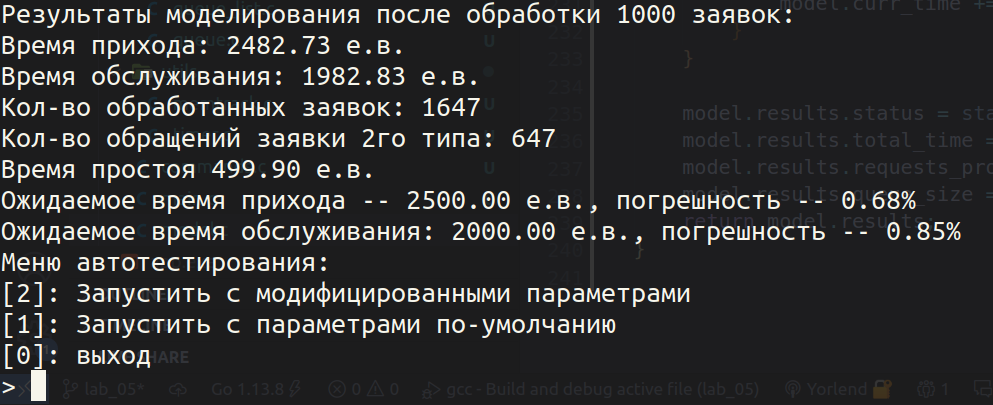
\includegraphics[width=0.7\linewidth]{img/model_res}
	\caption{Результаты работы модели с параметрами по-умолчанию}
	\label{fig:modelres}
\end{figure}

\section{Постановка эксперимента}

В данном эксперименте проводится сравнительный анализ эффективности работы реализаций очереди на основе кольцевого массива и линейного односвязного списка. Анализ проводится по времени работы и по объему затрачиваемой памяти.

\subsection{Технические характеристики}

Ниже представлены технические характеристики ПО, на котором производится тестирование ПО.

\begin{itemize}[$\bullet$]
	\item операционная система: Ubuntu 20.04 Linux 64-bit;
	\item оперативная память: 16 GB;
	\item AMD Ryzen 5 3500U with Radeon Vega Mobile Gfx @ 8x 2.1GHz;
\end{itemize}

\subsection{Описание экспериментальных данных}

Тестирование произведено на основе очередей, максимальный размер которых 50 элементов. Для тестирования временной эффективности будет произведено 10 замеров вставки-удаления, после чего результат будет усреднен.

\section{Результат эксперимента}

\subsection{Время работы}

В результате подсчета эффективности по времени для очередей на основе массива и списка, были получены следующие данные, отображенные в таблице \ref{tab:t}.

\begin{table}
	\caption{Время выполнения}
	\label{tab:t}
	\begin{center}
		\begin{tabular}{|c|c|c|}
			\hline
			Реализация очереди & Вставка, тики & Удаление, тики \\
			\hline
			Линейный список & 2853 & 2433 \\
			\hline
 			Кольцевой массив & 988 & 242 \\
 			\hline
		\end{tabular}
	\end{center}
\end{table}

Можно увидеть, что реализация очереди на основе линейного списка на 65\% эффективнее по вставке, и на 90\% эффективнее по удалению элемента.

\subsection{Затрачиваемая память}

В результате подсчета затрачиваемой под очереди памяти, были получены следующие результаты (таблица \ref{tab:m}).

\begin{table}
	\caption{Затраты памяти}
	\label{tab:m}
	\begin{center}
		\begin{tabular}{|m{7em}|m{5em}|m{7em}|m{7em}|m{10em}|}
			\hline
			Макс. размер & реал. размер & Объем памяти на кольцевом массиве, байт & Объем памяти списка, байт & относительная разница \% \\
			\hline
			10 & 0 & 32 & 24 & 79 \\
			\hline
			10 & 8 & 112 & 152 & -36 \\
			\hline
			100 & 15 & 832 & 264 & 68 \\
			\hline
			100 & 50 & 832 & 824 & 1 \\
			\hline
		\end{tabular}
	\end{center}
\end{table}

Исходя из приведенных выше данных, можно сделать вывод, что реализация очереди на линейном списке выгоднее реализации на кольцевом массиве при проценте фактической заполненности очереди менее 50\%. В общем же случае массив занимает меньший объем памяти, чем линейный односвязный список.

\section{Анализ фрагментации}

Рассмотрим очереди, с максимальным числом элементов 5. Заполним их значениями от 1 до 5 (рисунок \ref{fig:frag1})

\clearpage

\begin{figure}
	\centering
	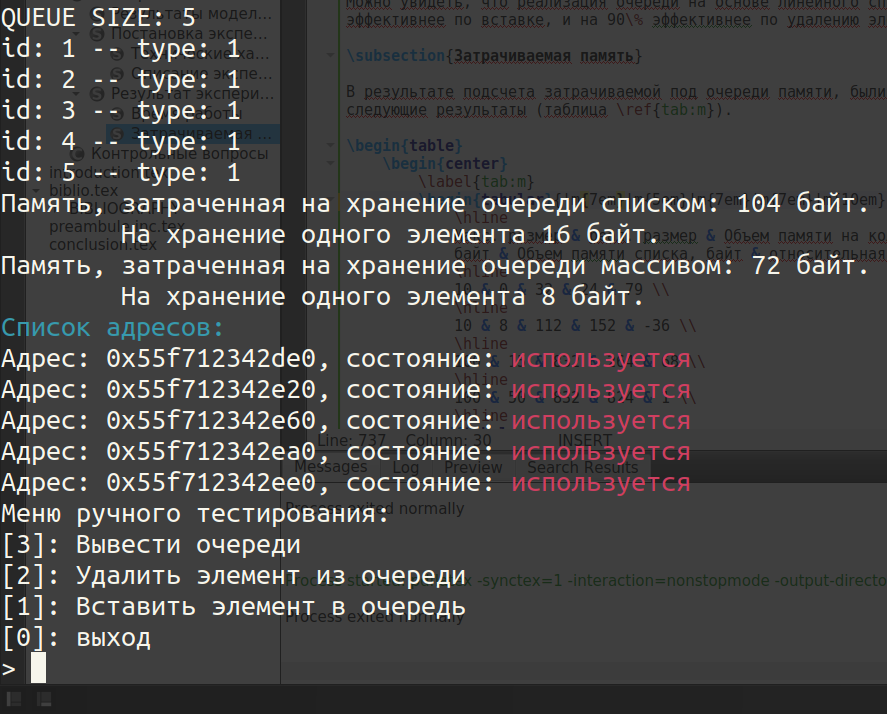
\includegraphics[width=0.6\linewidth]{img/frag1}
	\caption{Заполненные очереди}
	\label{fig:frag1}
\end{figure}

Удалим 2 элемента и вставим их снова (рисунок \ref{fig:frag2})

\begin{figure}
	\centering
	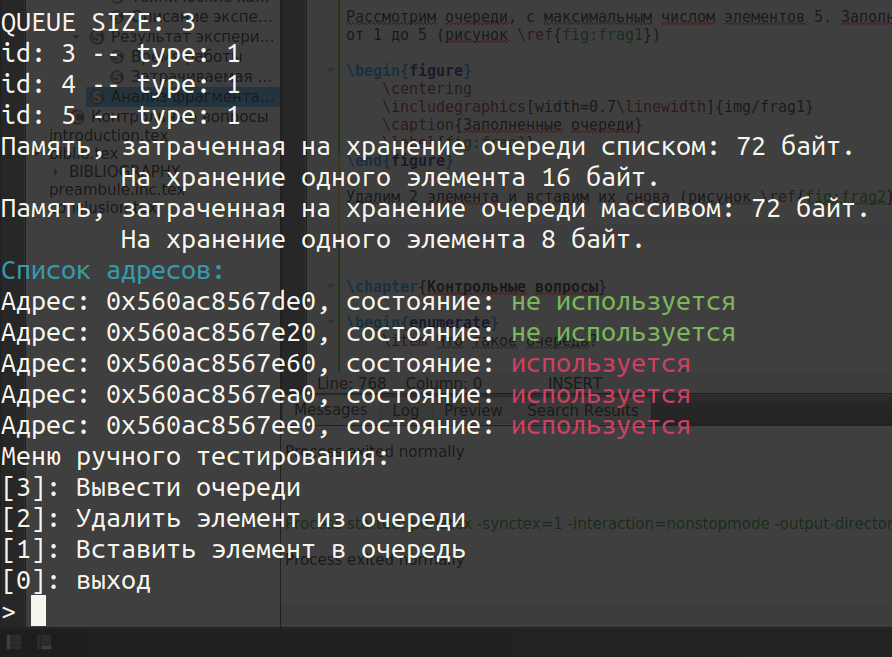
\includegraphics[width=0.6\linewidth]{img/frag2}
	\caption{Очереди из тремя элементами и двумя удаленными}
	\label{fig:frag2}
\end{figure}

\clearpage

Вставим эти элементы заново (рисунок \ref{fig:frag3})

\begin{figure}
	\centering
	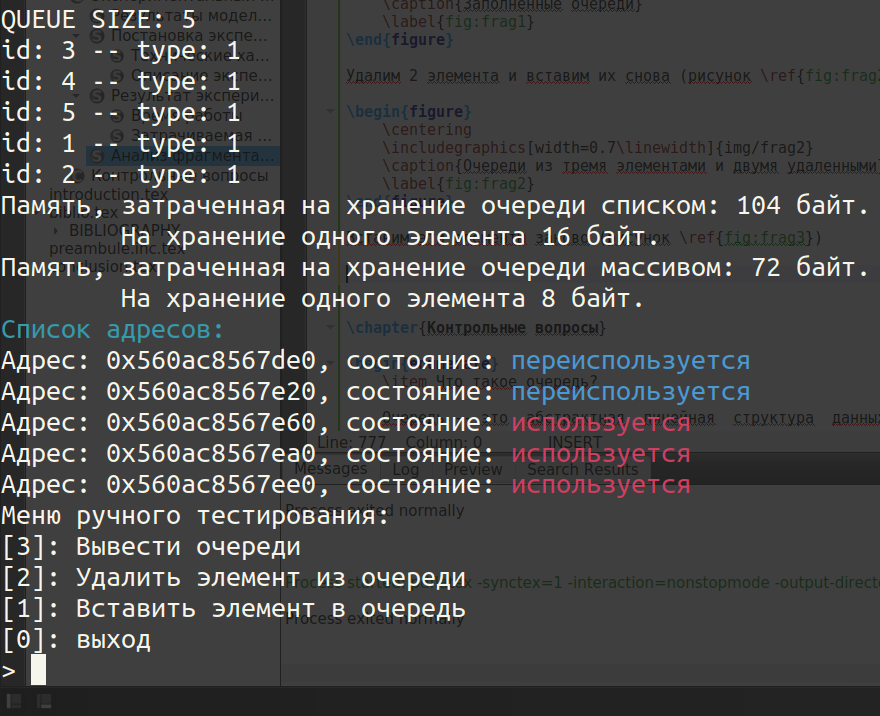
\includegraphics[width=0.6\linewidth]{img/frag3}
	\caption{Переиспользование областей памяти}
	\label{fig:frag3}
\end{figure}

Очистим и переинициализируем очереди (рисунок \ref{fig:frag4})

\begin{figure}
	\centering
	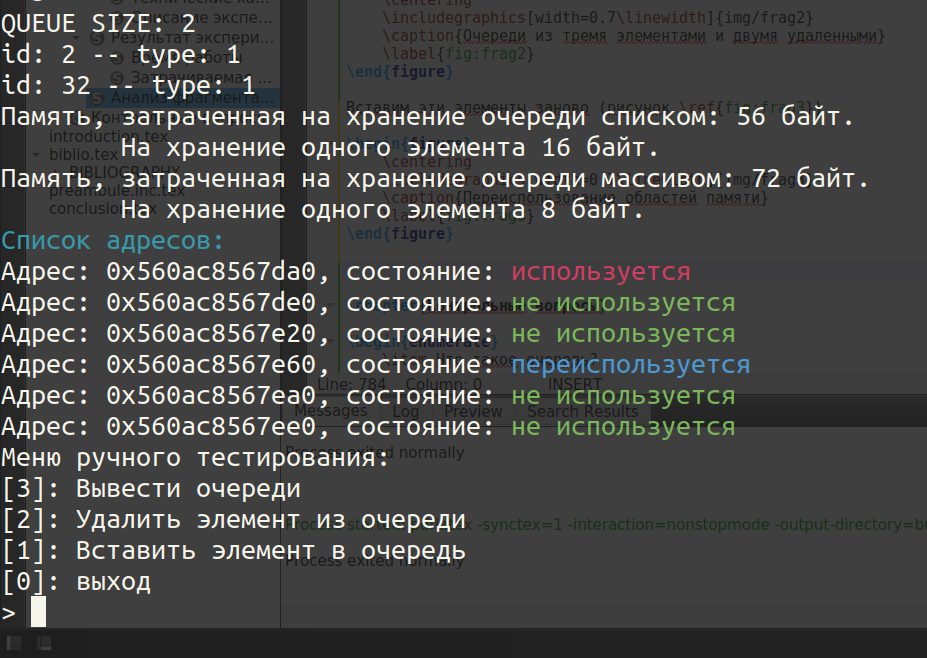
\includegraphics[width=0.6\linewidth]{img/frag4}
	\caption{Пустые очищенные очереди}
	\label{fig:frag4}
\end{figure}

\clearpage

Ниже, на рисунке \ref{fig:frag5}, можно заметить, что один из вставленных элементов переиспользовал ранее освобожденную память, а другой занял ранее неиспользуемую память.

\begin{figure}
	\centering
	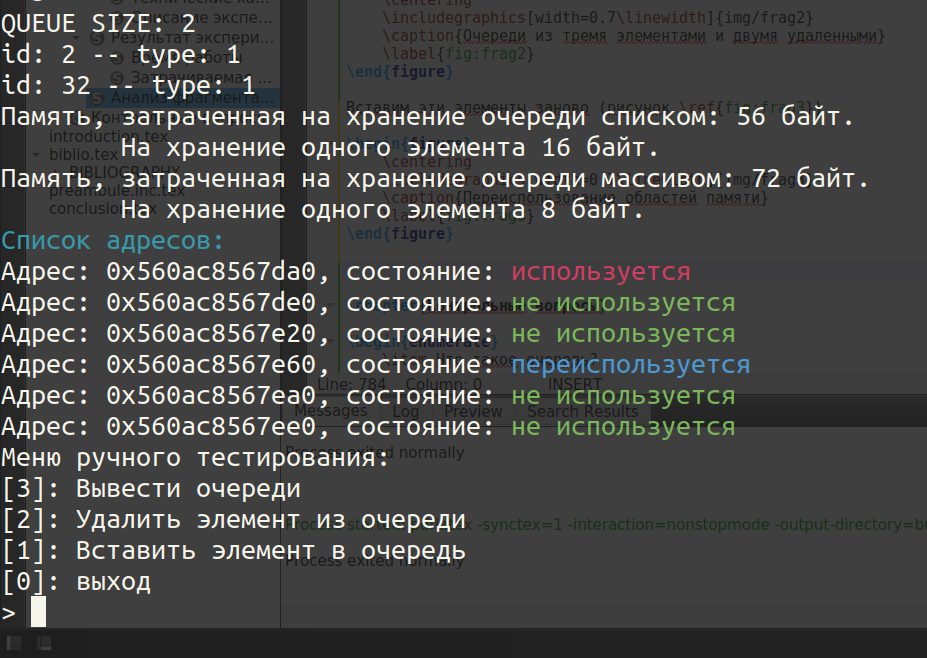
\includegraphics[width=0.6\linewidth]{img/frag5}
	\caption{Фрагментация}
	\label{fig:frag5}
\end{figure}

В результате чего наблюдаем фрагментацию памяти. Выделение цельного блока заданной длины не может быть произведено.


\chapter{Контрольные вопросы}

\begin{enumerate}
	\item Что FIFO и LIFO?
	
	Очередь работает по принципу FIFO  --  первый пришёл -- первый вышел. Стек работает по принципу LIFO -- последний пришёл -- первый вышел.
	
	\item Каким образом и какой объём памяти выделяется под хранение очереди при различной её реализации?
	
	При реализации очереди на массиве память выделяется  единожды в момент инициализации. 
	
	При реализации стека на связном списке память выделяется каждый раз при добавлении нового элемента в стек.
	
	\item Каким образом освобождается память при удалении элемента из очереди при её различной реализации?
	
	При  реализации  очереди  на  массиве  память  очищается  только  по окончании работы с очередью. 
	
	При реализации стека на связном списке память очищается каждый раз при удалении элемента из очереди. 
	
	\item Что происходит с элементами очереди при её просмотре?
	
	В  классической  реализации  очереди  просмотр  осуществляется поэлементным удалением элементов из одного конца, запоминанием их и вставкой в другой конец. 
	
	\item От чего зависит эффективность физической реализации очереди?
	
	Эффективность физической реализации очереди зависит от способа реализации очереди.
	
	\item Каковы достоинства и недостатки различных реализаций очереди в зависимости выполняемых над ними операций?
	
	Достоинства и недостатки реализации на массиве:
	
	\begin{itemize}
		\item[+] быстрота выполнения операций вставки и удаления;
		\item[---] нужно знать максимальный размер очереди заранее;
		\item[$\pm$] эффективна по памяти только при большой заполненности.
	\end{itemize} 
	 
	Достоинства и недостатки реализации на списке: 
	
	\begin{itemize}
		\item[+] размер ограничен лишь оперативной памятью;
		\item[---] операции выполняются медленнее, чем на массиве;
		\item[$\pm$] эффективна по памяти при небольшой заполненности.
	\end{itemize}

	\item Что такое фрагментация памяти, в какой части ОП она возникает?
	
	Фрагментация памяти -- явление, при котором занятые участки памяти перемешаны со свободными участками. Оно приводит к ситуациям, когда несмотря на то, что физический объем свободной памяти достаточен для выделения блока заданной длины, выделение не может быть осуществлено из-за отсутствия цельного свободного блока памяти заданного размера. Фрагментация возникает в куче (heap).
	
	\item Для чего нужен алгоритм <<близнецов>>?

	Метод близнецов необходим для эффективного выделения памяти.
	
	\item Какие дисциплины выделения памяти вы знаете?
	
	Дисциплины: самый подходящий, первый подходящий и метод близнецов.
	
	\item На  что  необходимо  обратить  внимание  при  тестировании программы? 
	
	При тестировании программы необходимо учесть как можно больше (а в  лучшем  случае  все)  классов  эквивалентности  для  входных  данных, убедиться,  что  100\%  написанного  кода  было  выполнено,  и  результат выполнения совпадает с ожидаемым. 
	Также  следует  вести  учет  потребления  программой  ресурсов, выделяемых операционной системой. Все ресурсы по окончании работы с ними должны быть возвращены системе в полном объеме.
	
	\item Каким образом физически выделяется и освобождается памяти при динамических запросах?
	
	При  запросе  на  выделение  памяти  менеджер  памяти  проходит  по списку  блоков  памяти  в  поисках  блока  требуемого  размера,  далее  если свободный блок слишком большой, он разбивает его на два, возвращая указатель на блок требуемой длины. Если же блок требуемого размера не был  найден  (например  вследствие  фрагментации  памяти)  то  менеджер памяти завершает работу с неудачей. 
	При  освобождении  памяти  менеджер  памяти  помечает  блок  как свободный и при необходимости объединяет соседние свободные блоки в один. 
	
	
\end{enumerate}

